\documentclass[margin 2cm]{report}
\usepackage{indentfirst}
\usepackage{setspace}
\usepackage{graphicx}
\usepackage{float}
\usepackage{url}
\usepackage{subfigure}
\usepackage{geometry}
\geometry{a4paper, scale=0.8}
\setcounter{secnumdepth}{4}
\title{\textbf{Codes and Cryptography Coursework}}
\author{zlqf46, 000785609}
\date{10/1/2021}
\begin{document}
\maketitle
\section[1]{\Large Part one: Compression}
\begin{enumerate}
\normalsize\item[1)]{Number Adaptive Encoding with 'big'}
\begin{spacing}{1.5}
\normalsize\indent\setlength{\parindent}{2em}As the LZ series and Huffman are all cumming out with the number sequence. And to prevent to write the number to the zip file directly. I Use the function $int.to_bytes(number, write_in_length, byteorder="big")$ to encode the int sequence into the certain bytes length to reduce the length waste, such as encoding the number \textbf{234} into byte b'\verb|\|xea', as the write in byte width is 1. Which greatly help shorten compressed number.
\end{spacing}

\normalsize\item[2)]{Length Adaptive Encoding}
\begin{spacing}{1.5}
\normalsize\indent\setlength{\parindent}{2em}Base on the first idea. The different int number has the different length of the encoding while write into the \textbf{.lz} file. I found that the length requirements are as follow:
\newline
\newline
\begin{tabular}{|l|c|r|}
\hline
$255<int<=65535$&$65535<int<=16777215$&$16777215<int$\\
\hline
width 2&width 3&width 4\\
\hline
\end{tabular}
\newline\normalsize\textbf{width 1 if the int smaller than 255}\\
By finding the biggest int number to decide which width is fix for encoding to reduce the compressing space.
\end{spacing}

\normalsize\item[3)]{Length Adaptive Encoding}
\begin{spacing}{1.5}
\normalsize\indent\setlength{\parindent}{2em}


\end{spacing}


\end{enumerate}


\newpage
\Large\section[2]{Cryptography}

\begin{enumerate}
\normalsize\item[1)]{Attack Plan}
\begin{spacing}{1.5}
\newline\normalsize\indent\setlength{\parindent}{2em}According to the FAQs\footnote[1]{\url{https://support.what3words.com/en/articles/2212810-what-are-the-shortest-and-longest-words-used}} on the whats3words wed page. I found that in English, the shortest words are four letters long and the longest words are 17-18 letters. And when trying the \textbf{encrypt.exe}, I also found that the input length of the Hexadecimal code is the same as the outputs (as shown in the example with "0123456789abcdef"). And the input codes length should be multiple of 8. \newline Mentioned in the coursework requirement, the length of the final outcome of the encryption is 32 bytes. And the key which in the \texbf{encrypt.exe} is the same while encrypting the outcome. \newline Thus, the input length of 3 words location should be 32 bytes after converting to hexadecimal. Each length of the words in the location string should be in range 4 to 18. And the result of the 3 words (in hexadecimal) from \textbf{encrypt.exe} should be the same as using the DES in ECB mode. So I will try to use the words in the word list to combine a 3 words location (using three 'for' loops) to encrypt it and compare it to the outcome. If it is the same, the location is found. For the coding part, I used the \textbf{multiprocessing.Pool} package. For the first word (in the first 'for' loop), separate the words list in few groups (run it in \textbf{Pool}) to combine with the second word (in the second 'for' loop)  and the third word (in the third 'for' loop). \newline\textbf{Material: 10k words list\footnote[2]{\url{http://www.mit.edu/~ecprice/wordlist.10000}}, 57k words list\footnote[3]{\url{https://raw.githubusercontent.com/dwyl/english-words/master/words_alpha.txt}}}
\end{spacing}

\begin{spacing}{1.5}
\normalsize\item[2)]{Step for Encryption through \textbf{encrypt.exe}}
\newline\normalsize\indent\setlength{\parindent}{2em}a) Encode the three words location (e.g. b'tile.bills.print') from bytes to hexadecimal which achieve the requirement length 32 bytes for \textbf{encrypt.exe}. \newline b) Encrypt the hexadecimal code using \textbf{encrypt.exe} and get the output. \newline c) Compare the output to the outcome from the coursework requirement.
\end{spacing}

\begin{spacing}{1.5}
\normalsize\item[3)]{Additional Finding}
\newline\normalsize\indent\setlength{\parindent}{2em}While encrypting the hexadecimal code. There are two points I found that can help to reduce the words number to reduce the searching time: a) When encoding the 3 words location from byte (e.g. b'tile.bills.print') to hexadecimal, the length of the hexadecimal code is twice the 3 words location. b) While encrypting through the \textbf{encrypt.exe}, the first 16 bytes of the outcome are the same if the first 8 letters (including the '.') are the same in the 3 words location. \newline\normalsize\indent\setlength{\parindent}{2em}According to the findings above and previous in Attack Plan. Firstly, the length condition for word chosen in 3 words location change to range 4 to 6. As the minimum words length is 4 and the  of the location should be exactly 16 (to require the 32 bytes length for hexadecimal and outcome), the longest word should no more than $16-2-4-4=6$\footnote[4]{which 2 for two '.', and 4 for the minimum length of the other two words}. Secondly, the searching area can be reduced by finding the first two words (reduce to two 'for' loops, randomly chose the third words) to compare the first 16 bytes of the encryption first. Then find out the first two words and use them to combine each word in words list (one 'for' loop) to find out the final word.
\end{spacing}

\begin{spacing}{1.5}
\normalsize\item[4)]{Attack}
\newline\normalsize\indent\setlength{\parindent}{2em}I first try with the 10k words list because it is the shortest one can finished earlier. By limited the 10k words list with the conditions behind, the number of the words can be reduced to 4k+8 words. So I separate it into 5 groups for the first loop (5 groups run in parallel using 8-core CPU with 16GB RAM on my Windows Laptop). After 280479s (around three days), the output of the first step are three combinations of the location, they are \textbf{"tile.bill.crimes", "tile.bills.catch","tile.billy.spies"}. \newline Then in the second step, use the word "tile" as the first word. Combine the word "bill" with 1504 words (length 6), "bills" with 1379 words (length 5), "billy" with 1379 words (length 5) which totally $1504+2\times1379=4262$ searches to encrypted by \textbf{encrypt.exe} and compare the outcome string. Fortunately, the 10k words list contain the third word "print" and the final answer for the 3 words is \textbf{"tile.bills.print"}.
\newline\textbf{The total running time is around 280479s+298s=281320s (78 hours). The total searches for the word is $4008^2+4262=16076088$. And the exactly location shows on Google Maps is: 7346 Melrose St, Philadelphia, PA 19136 US}
\end{spacing}

\begin{figure}[H]
\centering
\subfigure[first step time taken]{\label{Fig.sub.1}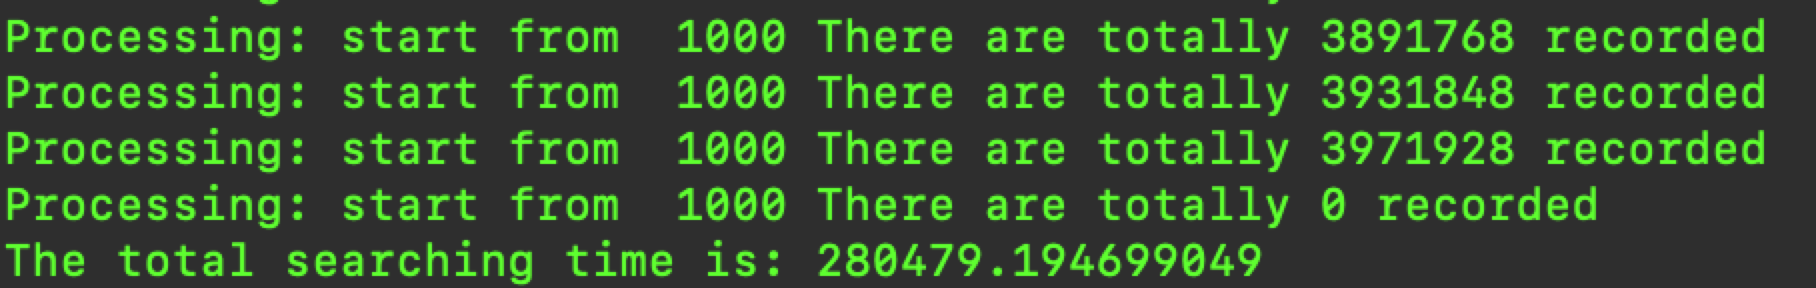
\includegraphics[width=0.5\textwidth]{evidence/time_taken_first_step.png}}
\subfigure[first step result]{\label{Fig.sub.2}\includegraphics[width=0.5\textwidth]{evidence/final_words.png}}
\subfigure[final result]{\label{Fig.sub.3}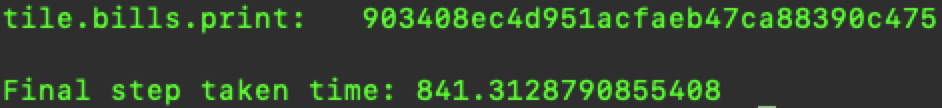
\includegraphics[width=0.5\textwidth]{evidence/final_location.png}}
\caption{Evidence}
\label{Fig.main}
\end{figure}

\normalsize\item[5)]{Evaluation and Fun Facts}
\newline\normalsize\indent\setlength{\parindent}{2em}As I found for reducing the words by the length limitation. There still have some improve in the first step like combining the words in a certain groups with certain length which can meet the length requirement of the words. And after finding out the 3 words location. I found that the \textbf{encrypt.exe} can be unpacked and find the key inside the \textbf{encrypt} file. Which is \texbf{'98a1bef23455dc03'}. And it works for encrypting the 3 words location with using the Des package in python.
\end{enumerate}


\end{document}